%%%%%%%%%%%%%%%%%%%%%%%%%%%%%%%%%%%%%%%%%
% Beamer Presentation
% LaTeX Template
% Version 1.0 (10/11/12)
%
% This template has been downloaded from:
% http://www.LaTeXTemplates.com
%
% License:
% CC BY-NC-SA 3.0 (http://creativecommons.org/licenses/by-nc-sa/3.0/)
%
%%%%%%%%%%%%%%%%%%%%%%%%%%%%


%----------------------------------------------------------------------------------------
%	PACKAGES AND THEMES
%----------------------------------------------------------------------------------------

%\documentclass[10pt]{beamer}
\documentclass[]{beamer}



\DeclareMathOperator*{\argmin}{arg\,min}


%%%%%%%%%%%%%

\usepackage{hyperref}


\newcommand{\bi}{\begin{itemize}}
\newcommand{\ei}{\end{itemize}}
\newcommand{\m}{\item}
\newcommand{\be}{\begin{enumerate}}
\newcommand{\ee}{\end{enumerate}}
\newcommand{\al}{\alert}
\newcommand{\ul}{\underline}


\mode<presentation> {

% The Beamer class comes with a number of default slide themes
% which change the colors and layouts of slides. Below this is a list
% of all the themes, uncomment each in turn to see what they look like.

%\usetheme{default}
%\usetheme{AnnArbor}
%\usetheme{Antibes}
%\usetheme{Bergen}
%\usetheme{Berkeley}
%\usetheme{Berlin}
%\usetheme{Boadilla}
%\usetheme{CambridgeUS}
%\usetheme{Copenhagen}
%\usetheme{Darmstadt}
%\usetheme{Dresden}
\usetheme{Frankfurt}
%\usetheme{Goettingen}
%\usetheme{Hannover}
%\usetheme{Ilmenau}
%\usetheme{JuanLesPins}
%\usetheme{Luebeck}
%\usetheme{Madrid}
%\usetheme{Malmoe}
%\usetheme{Marburg}
%\usetheme{Montpellier}
%\usetheme{PaloAlto}
%\usetheme{Pittsburgh}
%\usetheme{Rochester}
%\usetheme{Singapore}
%\usetheme{Szeged}
%\usetheme{Warsaw}

% As well as themes, the Beamer class has a number of color themes
% for any slide theme. Uncomment each of these in turn to see how it
% changes the colors of your current slide theme.

%\usecolortheme{albatross}
%\usecolortheme{beaver}
%\usecolortheme{beetle}
%\usecolortheme{crane}
%\usecolortheme{dolphin}
%\usecolortheme{dove}
%\usecolortheme{fly}
%\usecolortheme{lily}
%\usecolortheme{orchid}
%\usecolortheme{rose}
%\usecolortheme{seagull}
%\usecolortheme{seahorse}
%\usecolortheme{whale}
%\usecolortheme{wolverine}

%\setbeamertemplate{footline} % To remove the footer line in all slides uncomment this line
%\setbeamertemplate{footline}[page number] % To replace the footer line in all slides with a simple slide count uncomment this line

%\setbeamertemplate{navigation symbols}{} % To remove the navigation symbols from the bottom of all slides uncomment this line
}


%\setbeamertemplate{headline}
%{%
% \begin{beamercolorbox}{section in head/foot}
%\vskip1pt\insertnavigation{\textwidth}{}{}\vskip2pt
%  \end{beamercolorbox}
%}

\setbeamercolor{section in head/foot}{bg=lightgray} %set the top navigation bar background color
\setbeamertemplate{footline}[frame number] % set frame page number only
\usepackage{appendixnumberbeamer} % total will not include appendix frame numbers 

\beamertemplatenavigationsymbolsempty



\usepackage{graphicx} % Allows including images
% graphicx also allows for resizebox
% graphicx also allows for \scalebox
\usepackage{caption}
\usepackage{subcaption} % packgage for subcaption in subfigures
% The subfig and subcaption packages can not be used in cooperation with each other. Instead, you can usecaption package with subfig to add some flavor to the captions and subcaptions
\usepackage{bm} % make bold math symbols
\usefonttheme{professionalfonts}
%\usepackage{newtxtext,newtxmath} % for professional fond to load a Times Roman clone
\usepackage{tabularx} % extra features for tabular environment
\usepackage{booktabs} % Allows the use of \toprule, \midrule and \bottomrule in tables
\usepackage{adjustbox} % allows adjustbox
\usepackage{amsmath}  
\usepackage{amsfonts}
\usepackage{hyperref} % package for hyper link

% the following hypersetup makes link blue
\hypersetup{
  colorlinks   = true, %Colours links instead of ugly boxes
  urlcolor     = blue, %Colour for external hyperlinks
  linkcolor    = blue, %Colour of internal links
  citecolor   = blue %Colour of citations
}


\usepackage{float} % make the table H effective
\restylefloat{table}
\usepackage{color, colortbl}
\usepackage{booktabs} % package for tex professional table
\usepackage{mathtools} % package for \coloneqq
\usepackage{multirow} % multirow for intuition page.

% make pdf dark mode
%\usepackage{xcolor}
%\pagecolor[rgb]{0,0,0} %black
%\color[rgb]{0.5,0.5,0.5} %grey

\usepackage{pifont}% http://ctan.org/pkg/pifont
\newcommand{\cmark}{\ding{51}}%
\newcommand{\xmark}{\ding{55}}%



\usepackage{tikz} % graph in latex
\usetikzlibrary{positioning,arrows.meta} %tikz diagram
\usepackage{pgfplots}
\pgfplotsset{compat=newest} %this setting allow node to go to the correct place
\usepgfplotslibrary{fillbetween}

% use the tikz external library to cache tikz drawings
\usetikzlibrary{external}
\tikzexternalize[prefix=tikz/,optimize command away=\includepdf]


%\bibliography{bibliography}
%\usepackage[american]{babel}
%\usepackage{csquotes}
%\usepackage[style=apa]{biblatex}
%\DeclareLanguageMapping{american}{american-apa}
%\addbibresource{References.bib}

\usepackage{natbib} % package for citation


%\usepackage{subfigure} % subfigure package
%\captionsetup[subfigure]{labelformat=empty}
% The subfig and subcaption packages can not be used in cooperation with each other. Instead, you can usecaption package with subfig to add some flavor to the captions and subcaptions

%\usepackage{natbib} % package for citation

% define a comment line that does nothing to hide content
\newcommand{\comment}[1]{}
\newcommand{\lnb}[1]{%
  \ln\left(#1\right)%
}
\renewcommand{\baselinestretch}{1.0} %  scales the default interline space to 1.0 its default value. 

% define a comment that can scale the equation 
\newcommand\scalemath[2]{\scalebox{#1}{\mbox{\ensuremath{\displaystyle #2}}}}

%----------------------------------------------------------------------------------------
%	TITLE PAGE
%----------------------------------------------------------------------------------------

\title[Risk and Regulation]{\huge{Risk and Regulation} \\
\vspace{6mm}
\small{MGT 4074 Fintech \& Crypto Tokens, Fall 2025}
} % The short title appears at the bottom of every slide, the full title is only on the title page


%\subtitle{Presentation to Shanghai International Studies University}


\author[Joseph Hall]{Joseph Hall} % Your name
\institute[GT]{Georgia Institute of Technology} % Your institution as it will appear on the bottom of every slide, may be shorthand to save space
 % Your institution for the title page
 % Your email address
 
\date{October 20, 2025} 
 % Date, can be changed to a custom date if without date



%---------------------------------------------------------------------------
\begin{document}

\newcolumntype{d}[1]{D{.}{.}{#1}}


\begin{frame}
\titlepage % Print the title page as the first slide
\end{frame}


%----------------------------------------------------------------------------------------

%	PRESENTATION SLIDES
%----------------------------------------------------------------------------------------

%-----------------------------------------------



%---------------------------------------------------------------------
%---------------------------------------------------------------------
%\section*{Introduction}
% When I comment the introduction section, fewer sections show up in navigation
%---------------------------------------------------------------------
%---------------------------------------------------------------------



\begin{frame}{Welcome! Today is Monday 10/20/25}
\vfill 
\begin{center}


Today, I will discuss the  \textbf{Final Project}. Your \textbf{Final Project Proposals} are due on Wednesday 10/22!  

\end{center}
\vfill 

\end{frame}




\begin{frame}
\frametitle{Roadmap}
\tableofcontents
\end{frame}

%------------------------------------------------

%------------------------------------------------
% insert table of content before each section or subsection
%------------------------------------------------
\AtBeginSection[]
%\AtBeginSubsection[]
{
\begin{frame}
\frametitle{Roadmap}
\tableofcontents[currentsection,currentsubsection]
%\tableofcontents[currentsection]
\end{frame}
}
%------------------------------------------------


\section{Housekeeping}


\subsection{Midterm 2 Post-Mortem}

\begin{frame}{Good Job (on average)!}

The average score was again a solid B. By now, almost all of your grade besides the final project is in the books. 

\end{frame}

\begin{frame}{Margin Call Math}

\textbf{Q}: If you put \$50 into a \$125 position, what is your margin at that moment? \\ \pause 
\textbf{A}: 50/125 = 40\% \\ 
\textbf{Q}: How much does the stock price need to fall to bring the margin under 25\%? \\ \pause 
\textbf{A}: The broker is owed 125 - 50 = \$75. \textbf{That is a debt position so it gets paid first -- that is the number that won't change.} The broker's position is (1 - margin) of the total, so we are looking for \$75 to be (1 - 25\%) of what total? \pause Of \$100. So what needs to happen to the \$125 stock to make it worth \$100? \pause It needs to drop \textbf{20\%}. 
    
\end{frame}

\begin{frame}{AMM Math}

Short Answer 1 featured a \textbf{low-liquidity, low-fee} exchange and a \textbf{high-liquidity, high-fee} exchange and asked you to compare them for a \textbf{small trade} and a \textbf{large trade}. \\ \pause 

\begin{center}
    ``Intuition may fail you. The Math will never fail you'' \\ 
     -One of my PhD instructors 
\end{center}

Those of you who did the math correctly saw definitively that the fee matters more for the small trade, but liquidity matters more for the large trade. Small trade goes to Pool A, large trade goes to pool B. \\ 

Those of you who used intuition gambled and ended up with a wide variety of scores. 

\end{frame}


\subsection{Final Project}

\begin{frame}{Project Specification}

You will have two options for the final project: 

\bi 
\m \textbf{Build a Smart Contract}
\bi 
\m Create, deploy, and demonstrate the features of a smart contract 
\m Describe what failure of the traditional financial system this contract can address and why it is useful 
\m ``I have too few U.S. Dollars'' does not qualify (on its own) as a failure of the traditional financial system 
\ei 
\m \textbf{Defend a Mini-Thesis}
\bi 
\m Propose a \textbf{strong thesis statement} and at least one source of data to answer it 
\m Strong thesis statements (1) \textbf{matter} for society and the economy, and are (2) \textbf{controversial} ex-ante 
\m A policy proposal can fit into this category 
\m Your data may prove your statement right or wrong! 
\ei 
\ei 

    
\end{frame}

\begin{frame}{Groups}

You may work in groups of up to three students. If you do: 
\bi 
\m The expectations for the projects' scale and ambition will grow with the size of the group 
\bi 
\m A group of N choosing ``smart contract'' must create and demonstrate at least N interoperable and synergistic smart contracts with a total of at least 3N total functions 
\m A group of N choosing ``mini-thesis'' must analyze N distinct sources of data with at least 3N total data visualizations 
\ei 
\m There is no inherent advantage to working alone or in a group. Create a team if you trust your teammates to pull their weight. 
\m The project proposal must commit, in writing, to a \textbf{division of labor} ex-ante 
\ei 
    
\end{frame}


\begin{frame}{Proposals}

Proposals in my inbox \textbf{by start of class Wednesday 10/22}. 

\bi 
\m One proposal per group of up to 3 classmates 
\m Proposals must either (1) describe the functions your smart contract(s) will have or (2) describe the variables and observations in your dataset 
\m By Monday 10/27, I will announce the order of presentation. 
\m There are four presentation days scheduled (10/10 through 10/19). \textbf{The most ambitious projects (in my estimation) will go last}
\m Demos may be pre-recorded, but no student will escape live questioning 
\ei 
    
\end{frame}

\subsection{Post-Midterm Quiz Policy}

\begin{frame}{Quizzes}

From now until 11/5, \textbf{Pop Quizzes may include lecture content} \\ 

There is no more exam to study for, but you still need to pay attention in class! 
    
\end{frame}

\section{In the News}

\begin{frame}{Erebor Bank Approved by Regulators}

\begin{center}
    \href{https://x.com/tbpn/status/1978547597242744990}{3 Minutes from Technology Business Programming Network}
\end{center}

Crypto-friendly, digital-only bank named for LOTR dragon Smaug's hoard of gold will maintain hyper-conservative leverage ratio and focus on defense tech lending. 
    
\end{frame}

\section{Hacks}

\begin{frame}{Remember our friends at Infinifi?}

\begin{center}
    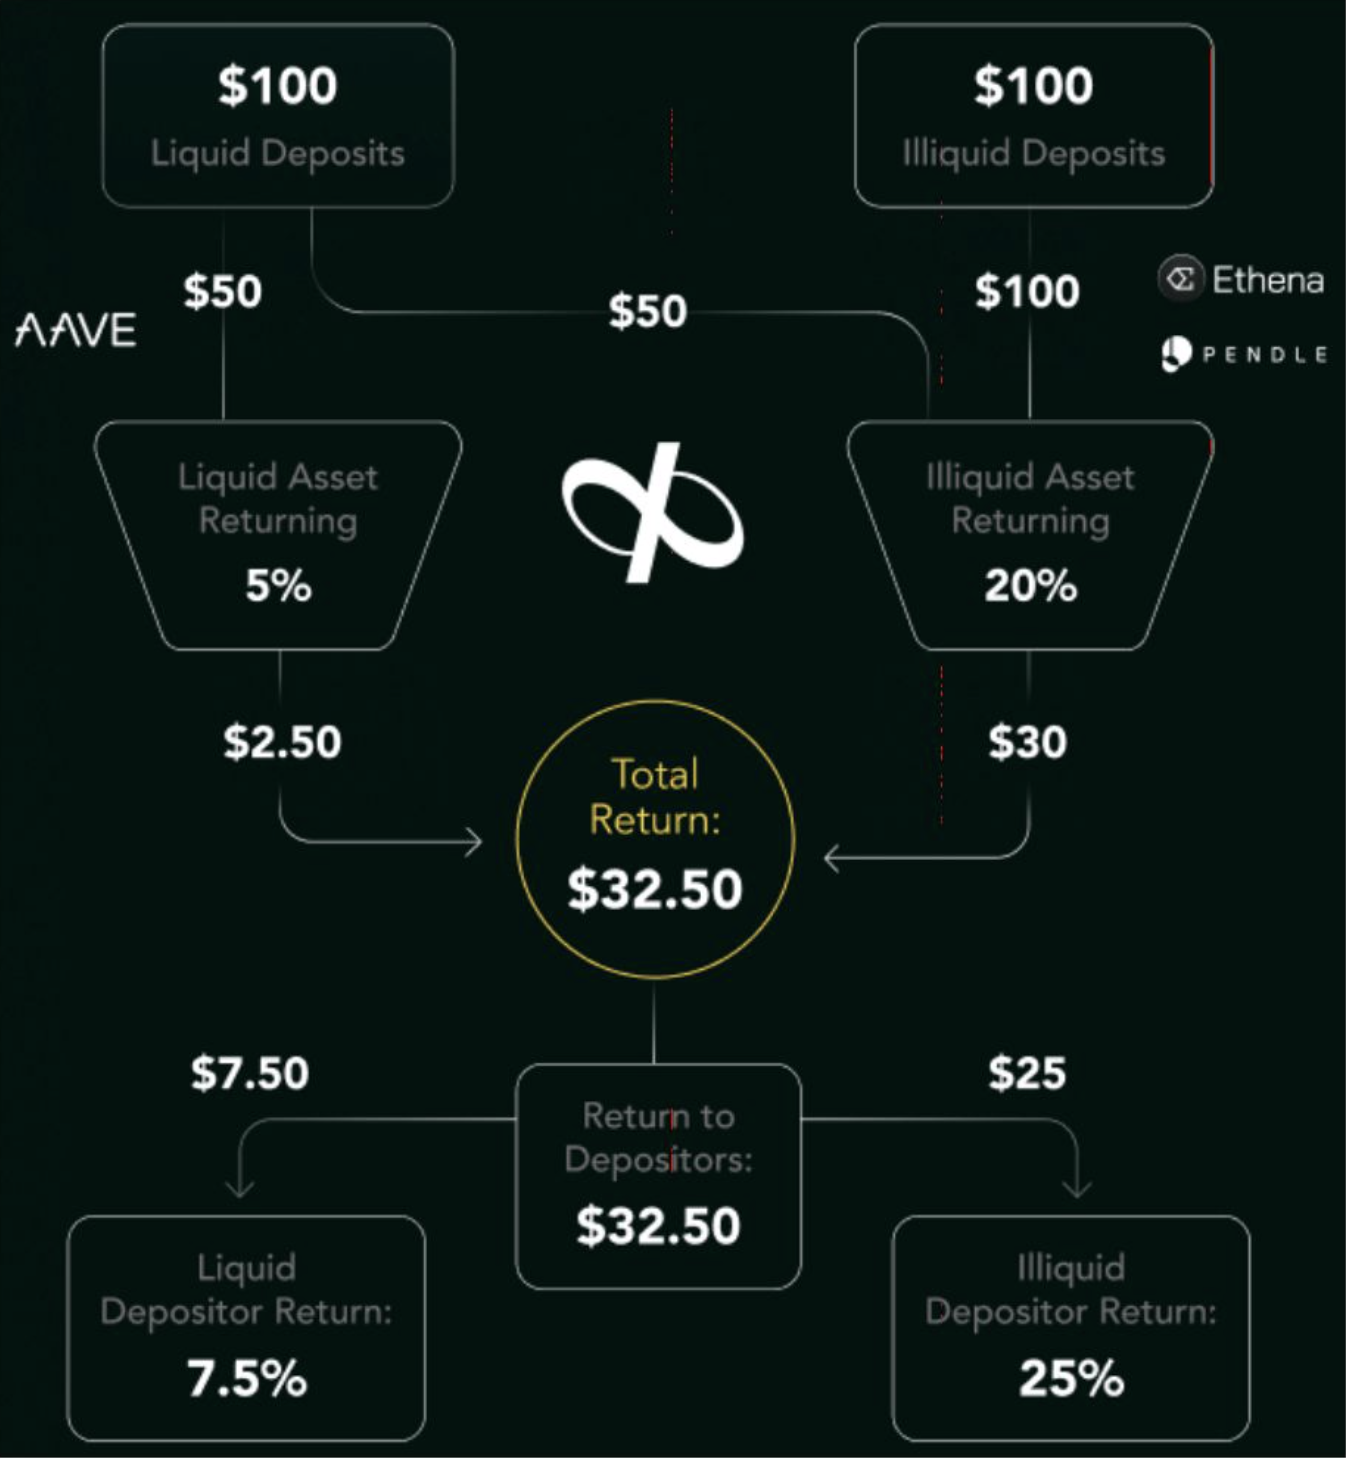
\includegraphics[height = 0.9\textheight]{infinifi.png}
\end{center}
    
\end{frame}

\begin{frame}{Treachery!}

\begin{center}
    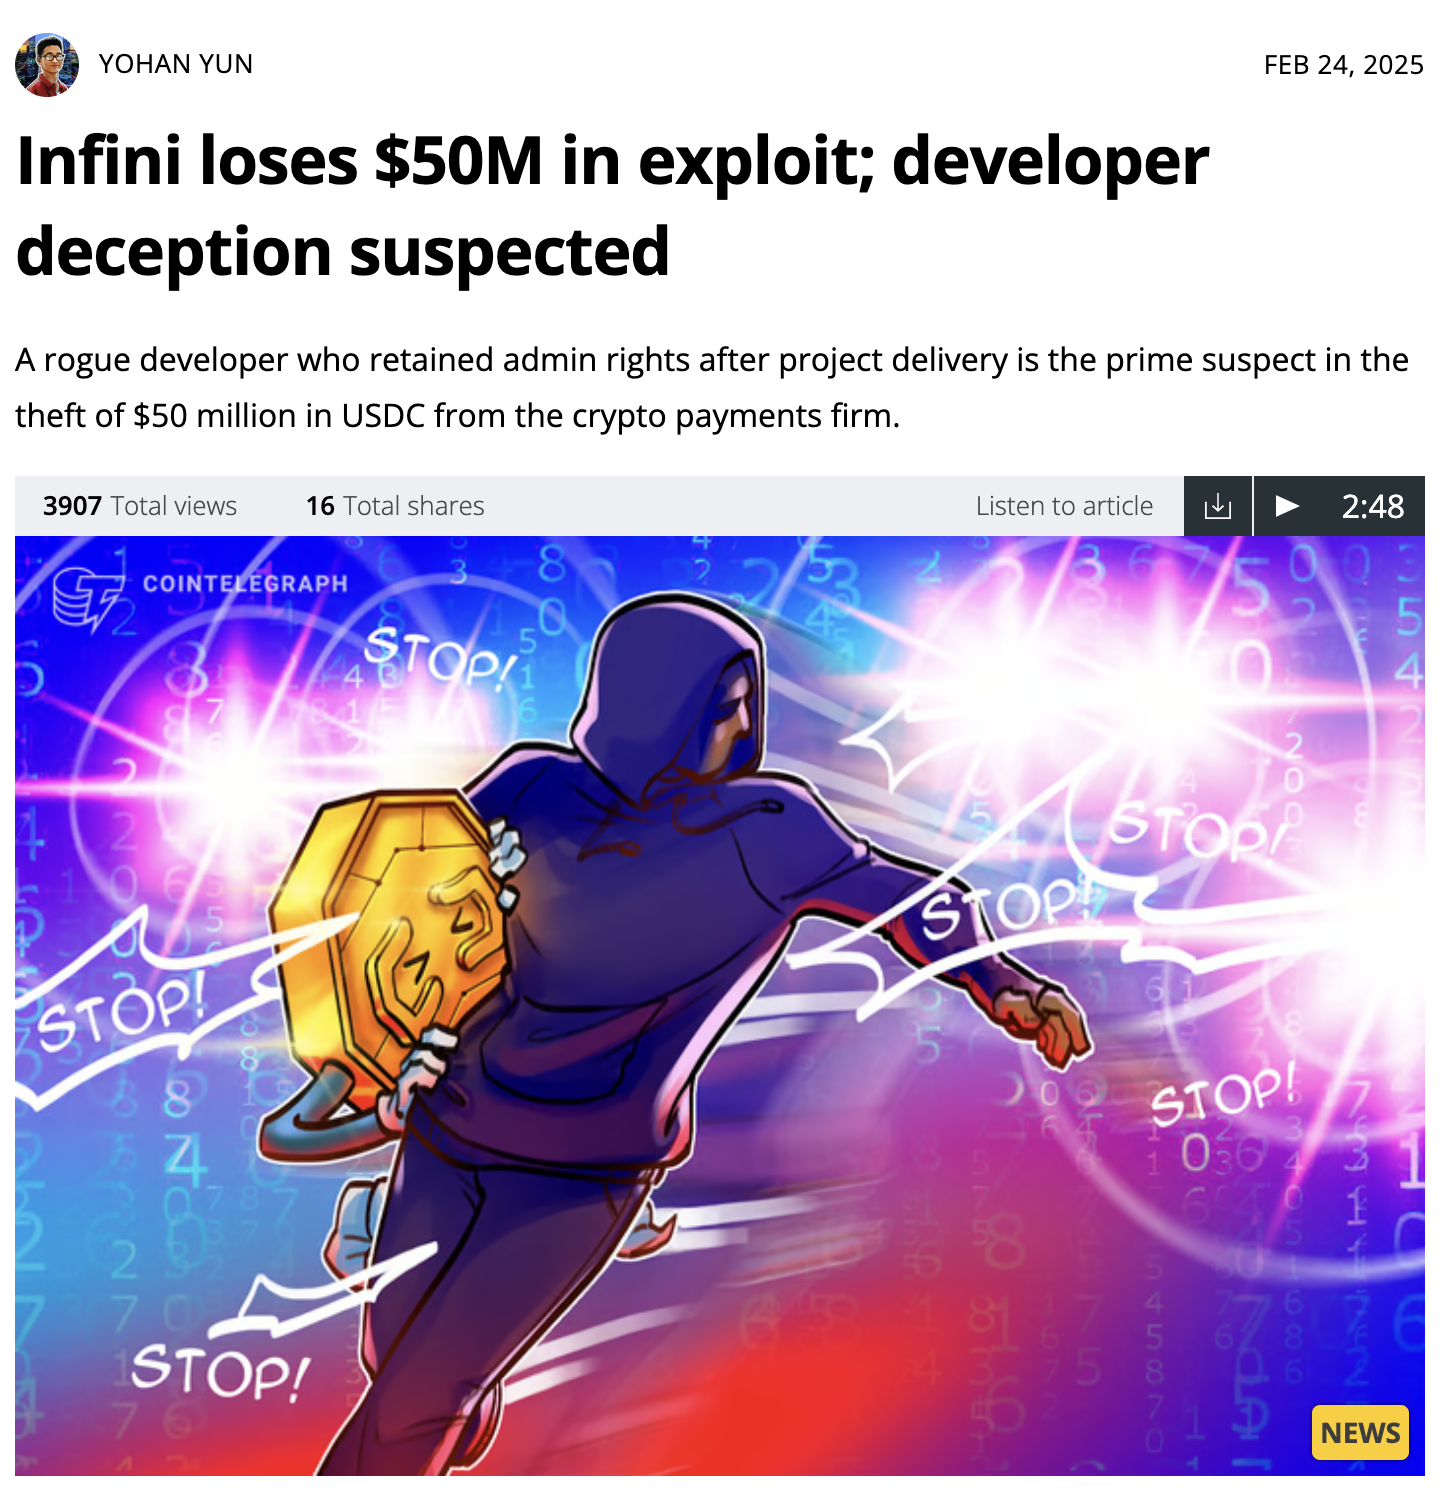
\includegraphics[height = 0.9\textheight]{yohan_headline.png}
\end{center}
    
\end{frame}

\begin{frame}{The Fate of All Crypto Exchanges is...}
\pause 

\begin{center}
    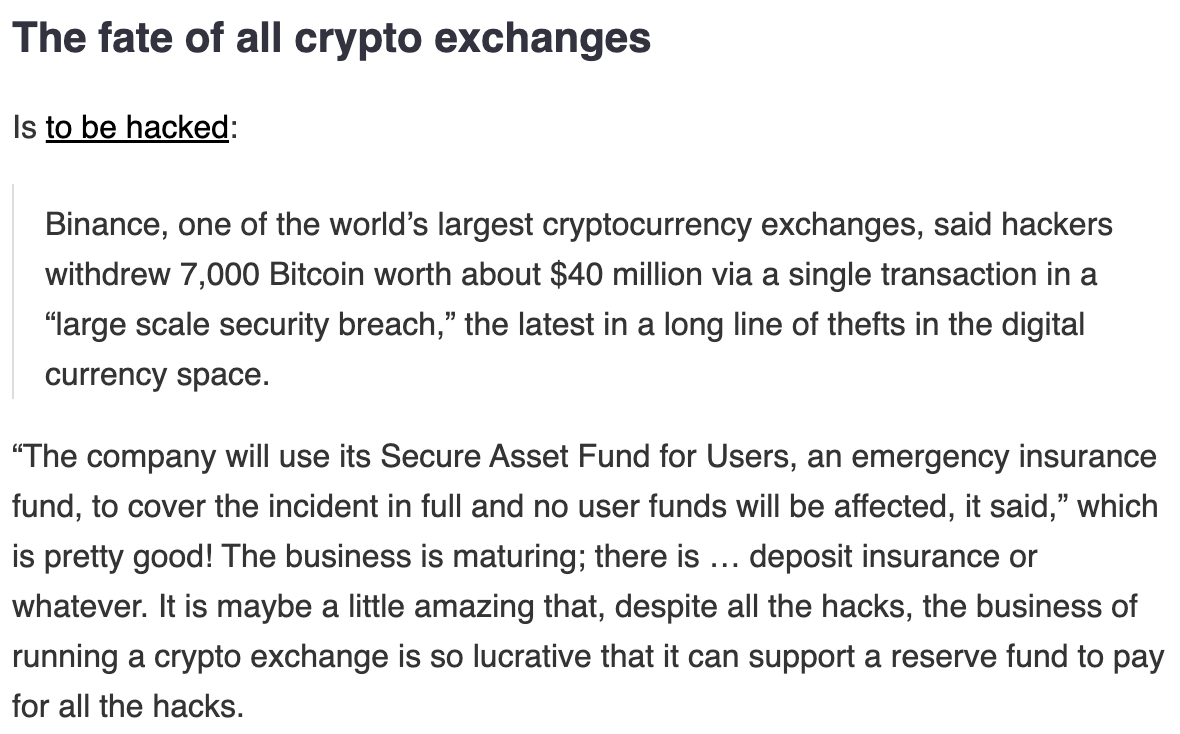
\includegraphics[width = 0.9\textwidth]{levine_fate.png}
\end{center}
From Matt Levine 
    
\end{frame}

\begin{frame}{Defending against code exploits}

Some strategies to defend against code exploits: 

\bi 
\m Change your passwords when you fire a disgruntled developer 
\m Write simple, immutable (non-upgradable) code 
\m Use bug bounty programs 
\m Employ `White Hat' hackers 
\m Trial and error, alpha/beta testing  
\m Read the news 
\ei 

\end{frame}

\begin{frame}{Morpho bug bounty via Immunifi}

\begin{center}
    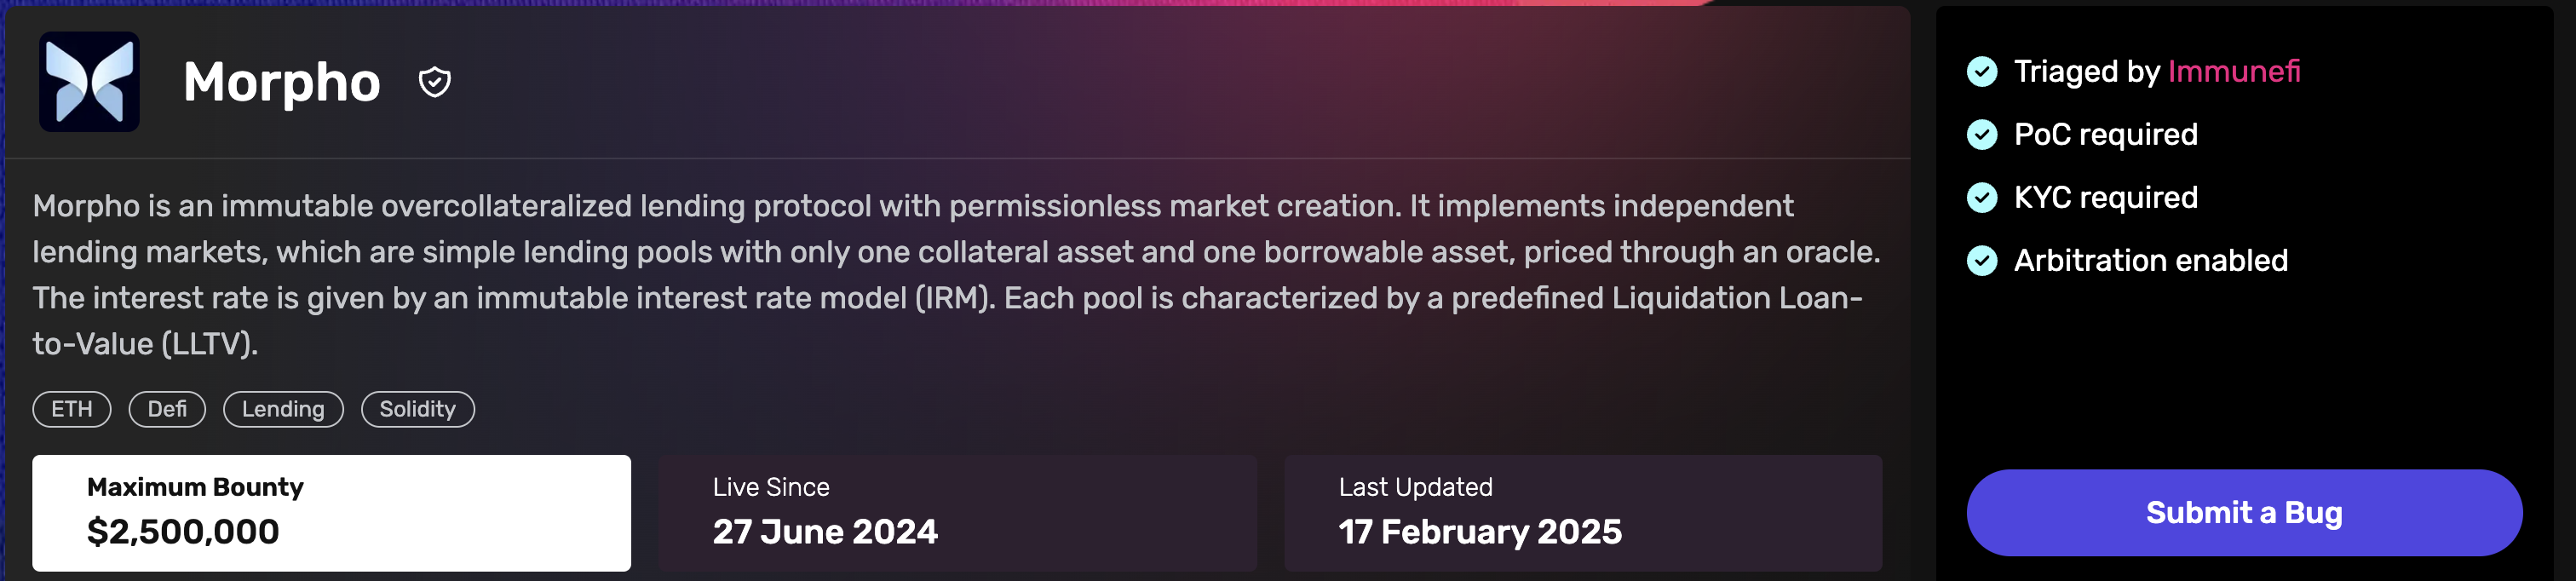
\includegraphics[width = \textwidth]{immunifi.png}
\end{center}

\bi 
\m Up to \$2.5M to find a ``critical'' bug in a Morpho smart contract
\m \href{https://immunefi.com/bug-bounty-program/}{Immunifi} has paid out \$115M in bug bounties with \$187M available today 
\ei 
    
\end{frame}


\section{Leverage}


\begin{frame}{Top Crypto Platform Coinbase Offers Leverage}

\begin{center}
    
\includegraphics[width = 0.9\textwidth]{coinbase_borrow.png}
\end{center}
    \bi 
    \m \textbf{Leverage}: borrow money to increase your risk + return 
    \ei 
\end{frame}


\begin{frame}{Coinbase partners with Morpho for margin lending}

\begin{center}
    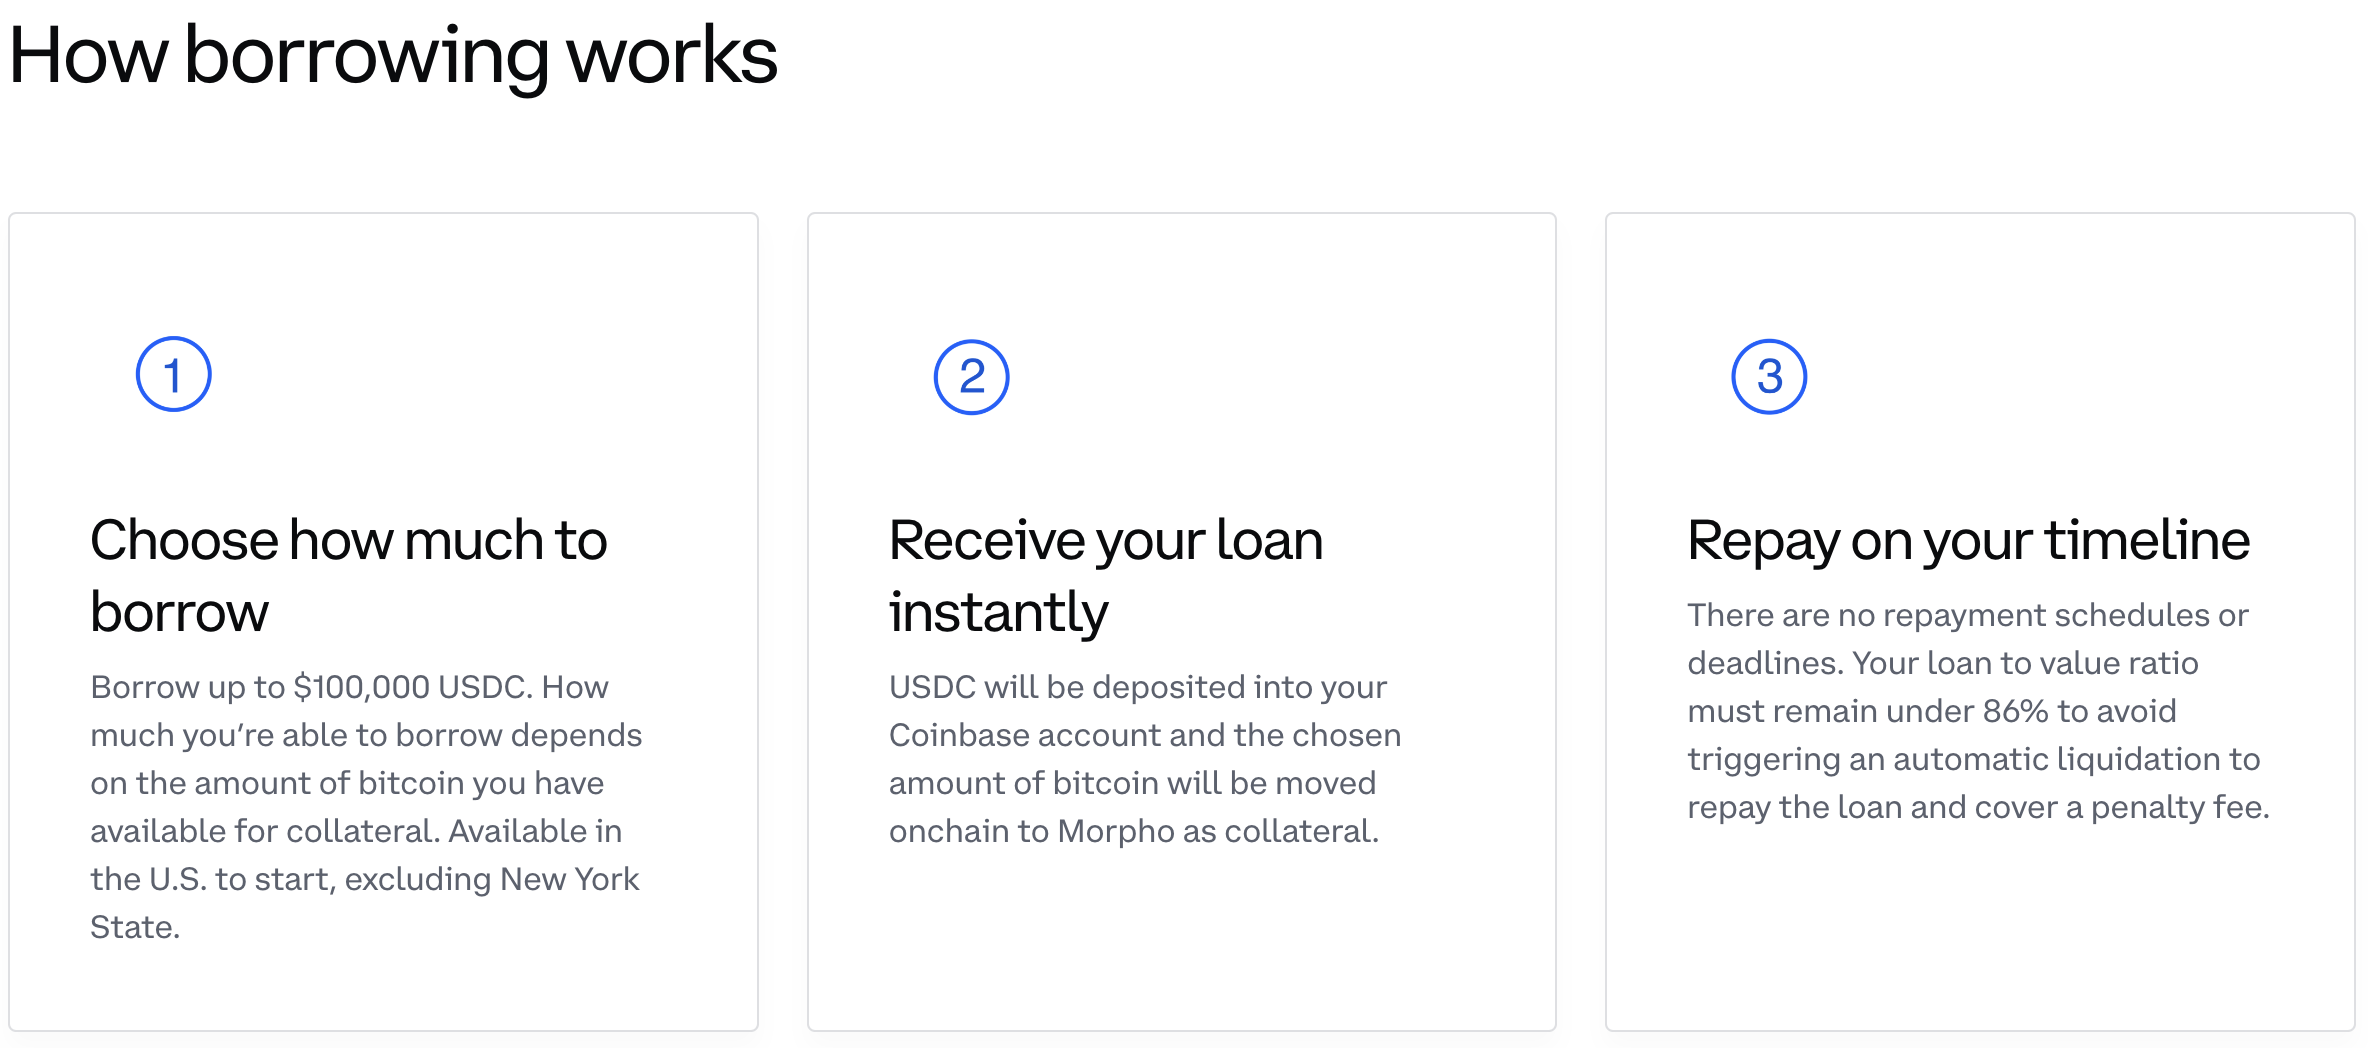
\includegraphics[width = 0.9\textwidth]{coinbase_morpho.png}
\end{center}
    
    
\end{frame}


\begin{frame}{Morpho Borrowing Rates and LTVs}


\begin{center}
    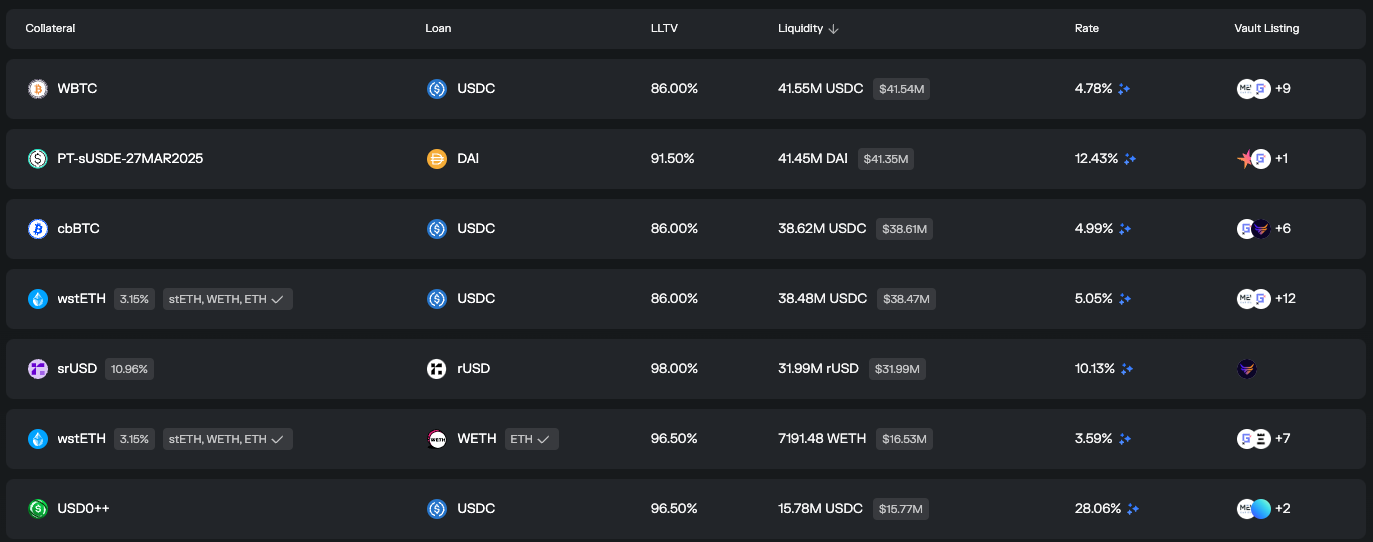
\includegraphics[width =\textwidth]{morpho_rates.png}
\end{center}

86\% LTV is only 14\% margin, lower than most mortgages and lower than FINRA minimum for tradfi margin trading 
    
\end{frame}

%\begin{frame}{Morpho Lending Rates}

%\begin{center}
%    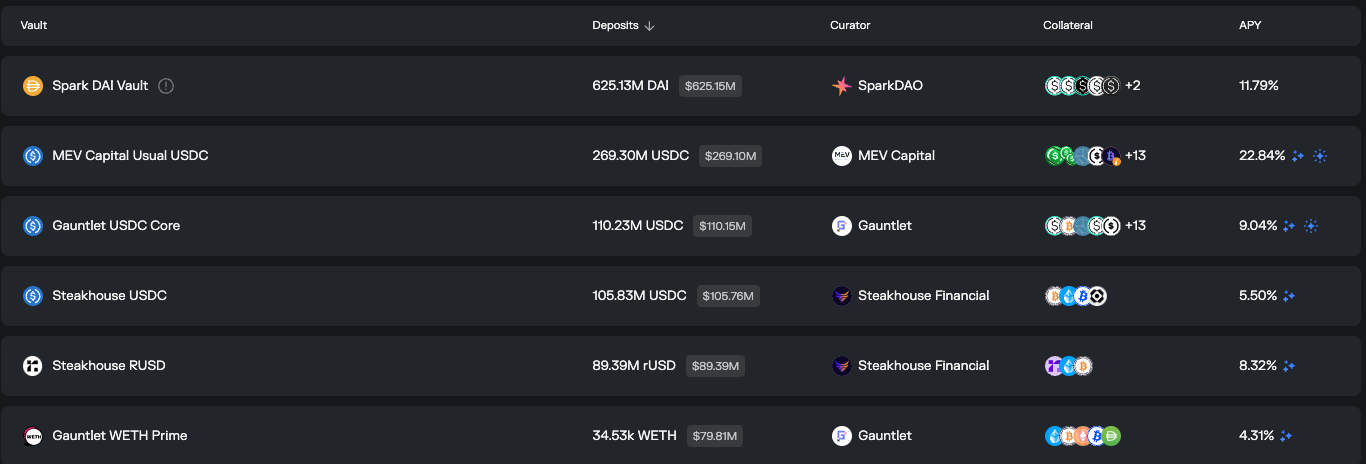
\includegraphics[width = \textwidth]{morpho_lenders.png}
%\end{center}

%How are lenders be earning 10-20\% while borrowers are paying 4-15\%? 
    
%\end{frame}

\begin{frame}{Morpho liquidation policy}

\begin{center}
    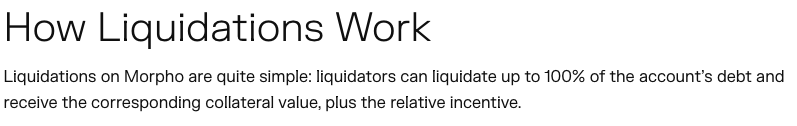
\includegraphics[width = \textwidth]{morpho_policy.png}
\end{center}
\pause 
As opposed to the \emph{Ajna Protocol} which leans \emph{against} spurious liquidations, the Morpho Protocol \emph{encourages} liquidations $\rightarrow$ \emph{Morpho Protocol} is friendly to creditors but punitive to borrowers \vfill \pause 

\href{https://coinalyze.net/morpho/liquidations/}{\$110k} of liquidations on the Morpho platform in the past 24h alone (as of when I wrote these slides)! 
    
\end{frame}

\begin{frame}{Crypto's ``Black Friday'' on 10/10/25}

On 10/10/25, over 200 altcoins (tokens that are not stablecoins, ETH, nor BTC) dropped by more than 80\% 

\begin{center}
    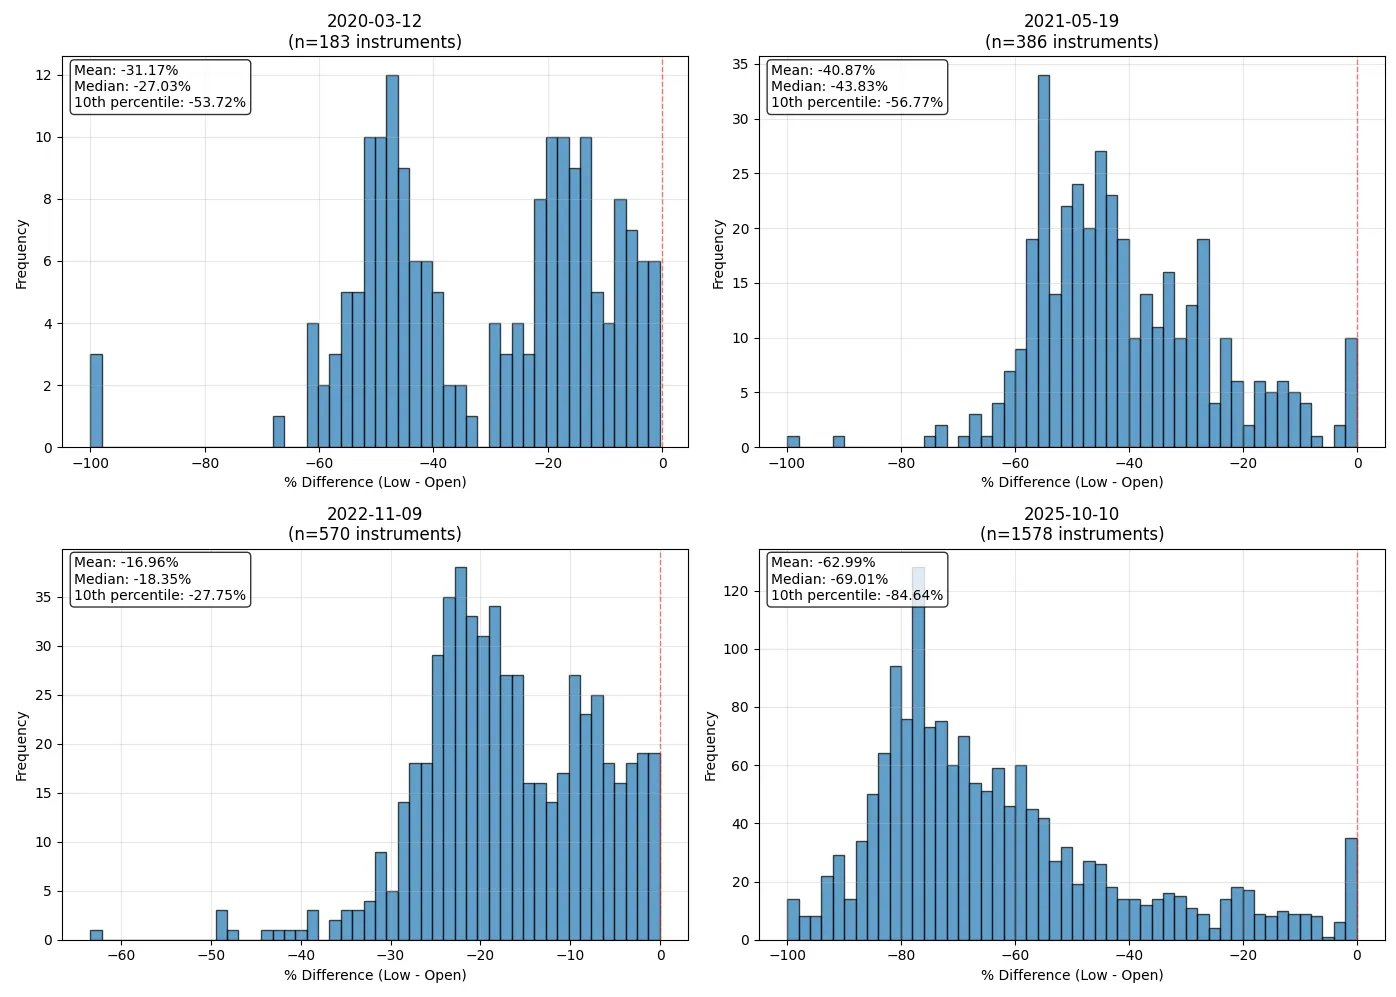
\includegraphics[width = .7\textwidth]{crypto_crash.jpeg}
\end{center}

Over \$19 \textbf{billion} of leveraged positions were liquidated in a matter of seconds (\href{https://x.com/ltrd_/status/1978161988196004285}{ltrd}) 
    
\end{frame}

\begin{frame}{Perpetuals}

A \textbf{Perpetual Futures Contract} (or ``perp'') is a zero-sum derivative contract between two market participants \\ 

One side bets the price of the underlying will go up, the other side bets it will go down \\

No one actually needs to touch the underlying asset! Just read the price of it off of an exchange. This has two implications: 

\bi 
\m Any amount of leverage is equally easy to implement: just multiply the price changes by 2x, 20x, 50x... 
\m The price of the underlying can go arbitrarily high: the short leg is always at risk of going below zero at \emph{any} leverage ratio above zero  
\ei 

Perp sellers are historically called ``bucket shops'' because they put traders' cash in a bucket, and traders just swap around the money in the bucket without touching the underlying.  

    
\end{frame}

\begin{frame}{Leveraged Perps}

\begin{center}
    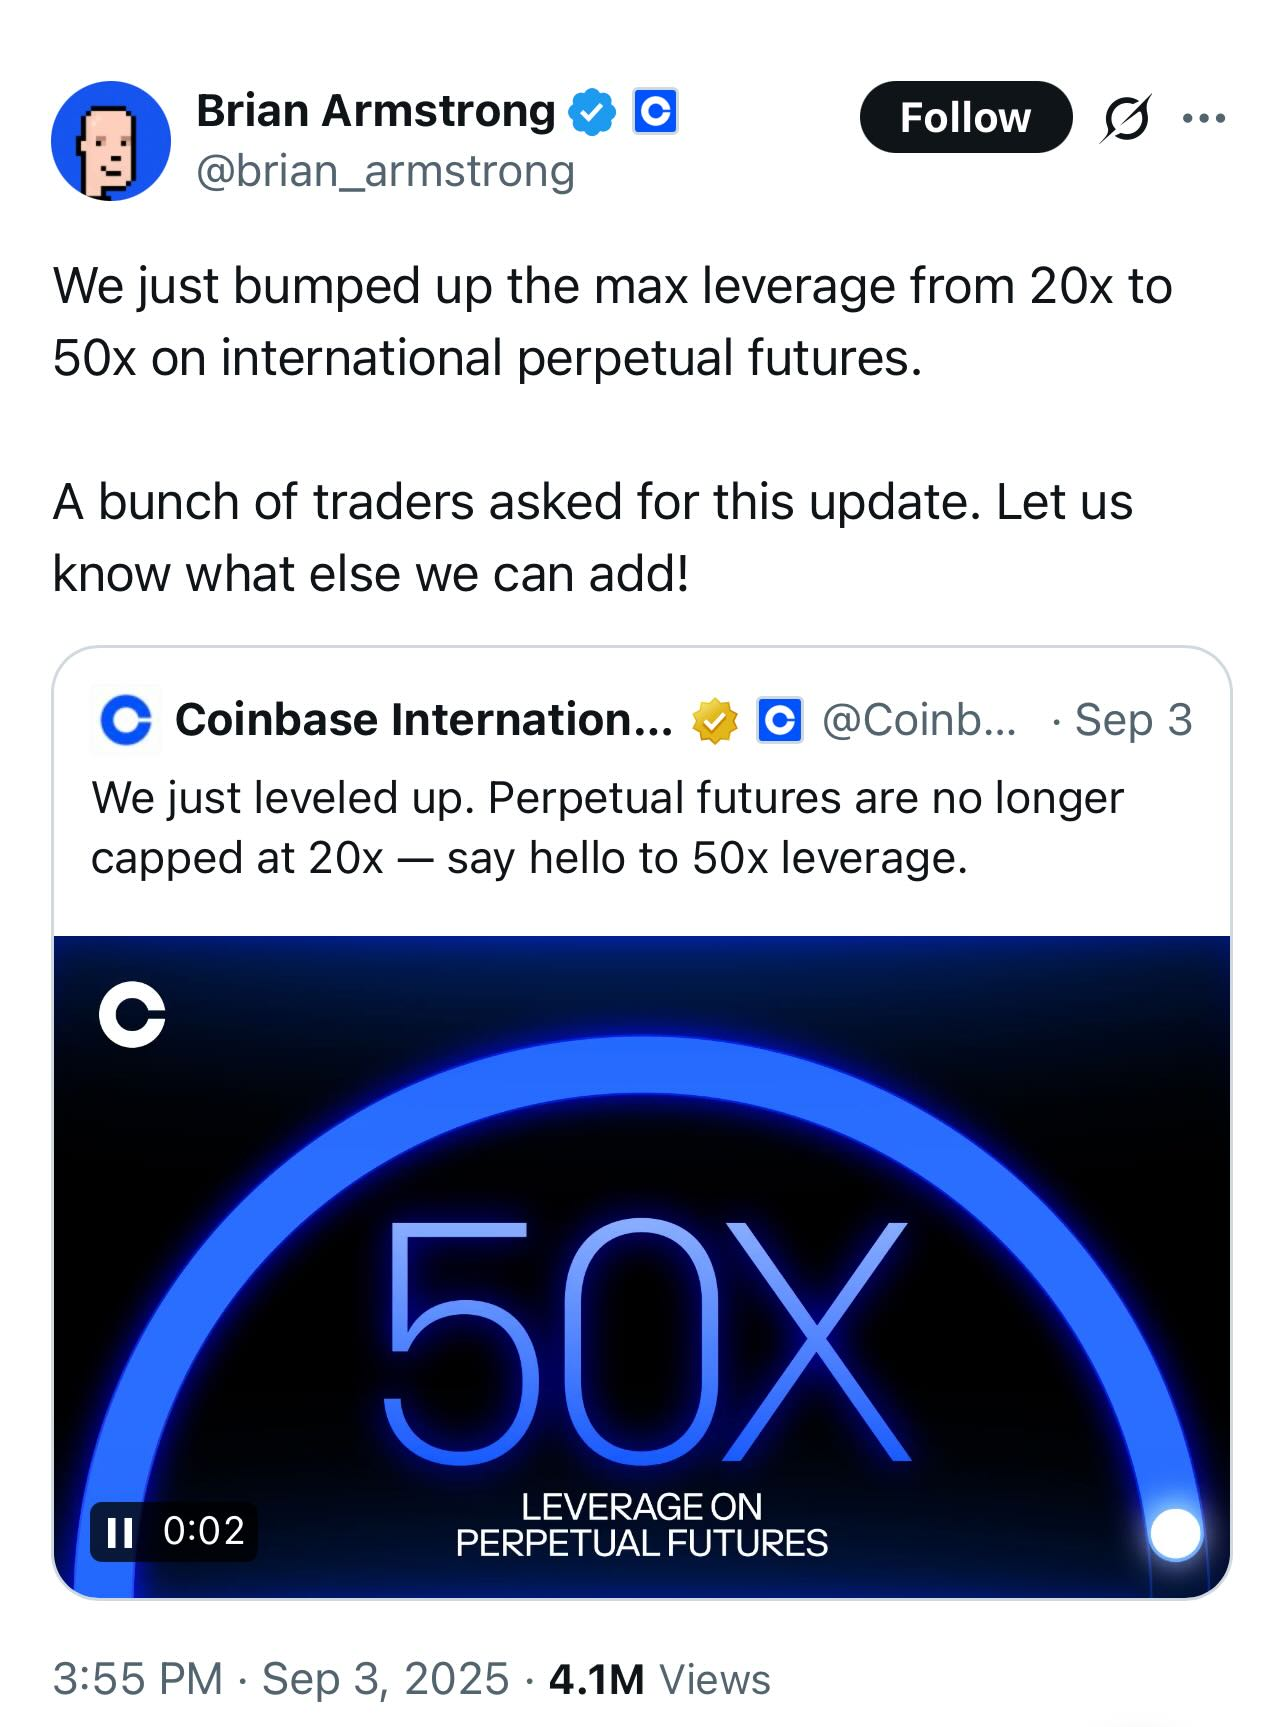
\includegraphics[height = .9\textheight]{50x_perps.jpg}
\end{center}

\bi 
\m Key question: what happens when a trader loses more money on a perp than they have deposited into their brokerage account? 
\ei 
    
\end{frame}

\begin{frame}{Auto-Deleveraging}

What happens when I win \$100 from you, but you only deposited \$50 into your brokerage account? \\ 

\textbf{Auto-Deleveraging} is when winning bets are closed early because their counterparty has gone bust. \\ 

On 10/10/25, \$19B of positions were hit by ADL. \\ 

Many traders use perps to \textbf{hedge} their exposure: If I'm long bitcoin, I short some leveraged bitcoin perps so that if my long position loses my short position will make up for it. \\ 

\textbf{Auto-Deleveraging} presents a threat to hedging strategies: if I'm long the underlying but short the perp, and the price falls a lot, my long position has lost but my winning position gets closed early! \\

Even worse: these traders need to find a new way to get short to stay hedged, pushing prices down further. 

\end{frame}

\begin{frame}{Crypto Black Friday}

Two other points bear mentioning: 
\bi
\m Reported liquidations on centralized exchanges like Binance may not be accurate. Liquidations reported by on-chain exchanges like \href{https://app.hyperliquid.xyz/trade/BTC}{Hyperliquid} are more trustworthy (\href{https://x.com/chameleon_jeff/status/1977578610329534958}{chameleon\_jeff}). 
\m Some traders have private deals with exchanges to avoid deleveraging! These private deals represent a hidden cost/subsidy from traders with out these deals (\href{https://x.com/darkmarketio/status/1977766731188740134}{darkmarketio}). 
\ei 
    
\end{frame}

\section{Regulation}


\begin{frame}{The GENIUS Act}

\begin{center}
    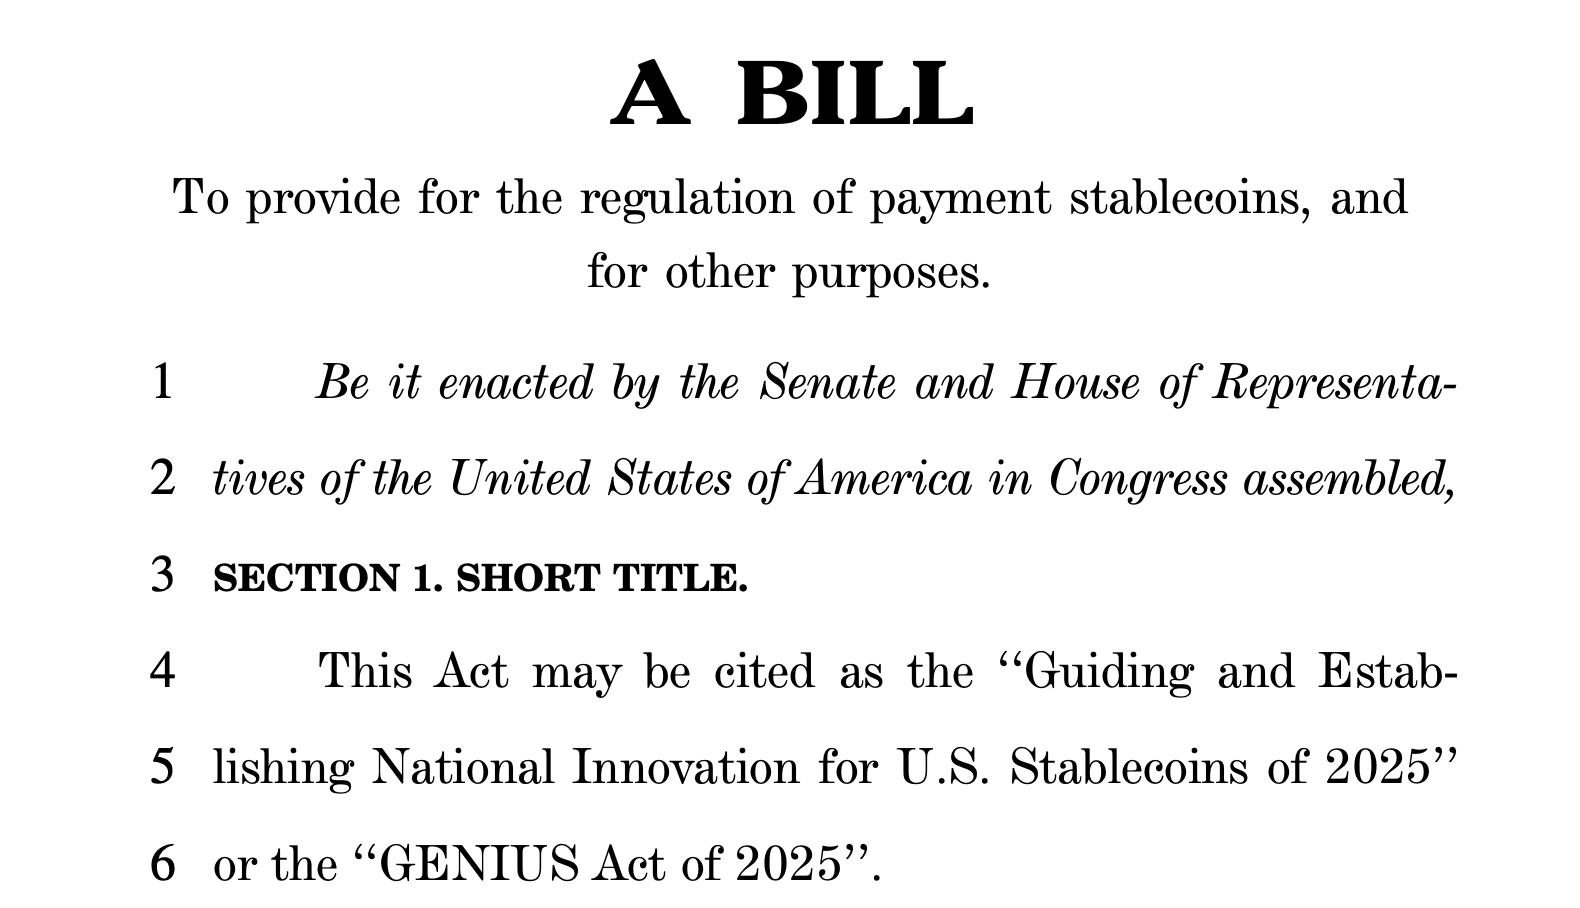
\includegraphics[width = 0.8\textwidth]{genius.png}
\end{center}

Introduced by Bill Hagerty (R-TN) \href{https://www.hagerty.senate.gov/wp-content/uploads/2025/02/GENIUS-Act.pdf}{(Full Text)}
    
\end{frame}

\begin{frame}{GENIUS Act}

The GENIUS Act: 
\bi 
\m Grants regulated issuers \textbf{exclusive} rights to distribute stablecoins 
\m Regulates sc issuers like banks at the federal \textbf{or state level}
\bi 
\m Issuers with \$10b+ assets \underline{must} register federally 
\ei 
\m Clarifies that stablecoins are \emph{not} ``securities'' (in the 1936 securities exchange act meaning) 
\m Requires ledgers to be \underline{public} to qualify as ``stablecoins'' 
\m Applies consumer protection laws to stablecoin wallet providers 
\m Prohibits paying interest on stablecoins (so they cannot compete with bank deposits) 
\ei 

Among other details (see \href{https://www.davispolk.com/insights/client-update/stablecoin-bill-first-out-gate-crypto-legislation-gains-momentum}{discussion by law firm Davis Polk}) 

\end{frame}


\begin{frame}{Prosecutorial Discretion}

\begin{center}
    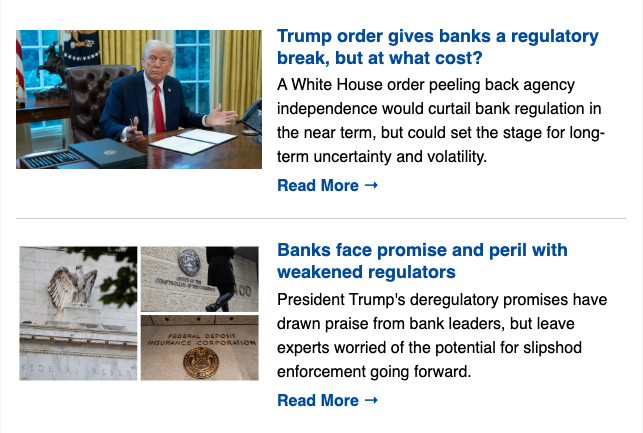
\includegraphics[width = .9\textwidth]{american_banker.png}
\end{center} 
Source: American Banker Newsletter 
\end{frame}


\begin{frame}{Prosecutorial Discretion}

\begin{center}
    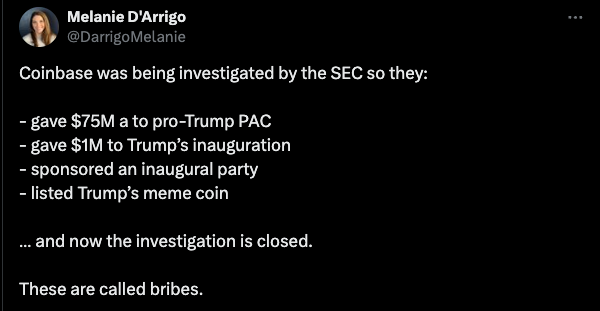
\includegraphics[width = \textwidth]{coinbase_bribes.png}
\end{center} \pause 
``Code is law''? How about ``Trump is law''?

\end{frame}


\begin{frame}{Meme-coin company bids on InfoWars}

\vfill 
Right-wing conspiracy theory and misinformation website InfoWars, founded by Alex Jones, must be sold to pay his legal liabilities stemming from Sandy Hook defamation case. \\ \vfill 

Meme-coin company Wow.ai has entered a bid to buy InfoWars using equity tokens. 
\vfill 
\end{frame}

\begin{frame}{Meme-coin company bids on InfoWars}

``We will receive proposals from people and entities who want to operate the website and Wars token-holders will get to vote on what decision to make,'' Infowars CEO Rick Latona said. ``So the creditors will be in an interesting situation because if this thing plays out over a year they have been invested in a lot of tokens.''
    
\end{frame}

\begin{frame}{Completing incomplete markets}

\begin{center}
    
\includegraphics[width = \textwidth]{arpit_gupta.png}
\end{center}

\bi 
\m Will wow.ai bring Arpit's idea to fruition? 
\ei 
    
\end{frame}


\end{document}